\documentclass[A4]{article}
\usepackage{graphicx}
\usepackage[hidelinks]{hyperref}
\usepackage{wrapfig}
\usepackage{xcolor}

\renewcommand{\familydefault}{\sfdefault}

\pagenumbering{gobble}

\hypersetup{
	colorlinks,
	linkcolor={red!50!black},
	citecolor={blue!50!black},
	urlcolor={blue!80!black}
}

\begin{document}
	\title{Usages of Light Shafts}
	\date{}
	
	\maketitle
	
	\section*{What are Light Shafts?}
	\textit{Light Shafts} are used for volumetric light and shadow effects. In this case, it stands for two different methods that are emulating crepuscular rays. These beams, often called \textit{Godrays}, appear when the atmosphere is saturated with aerosols where the incoming sunlight is scattered heavily.
	\begin{wrapfigure}{r}{0.5\textwidth}
		\begin{center}
			\vspace{-20px}
			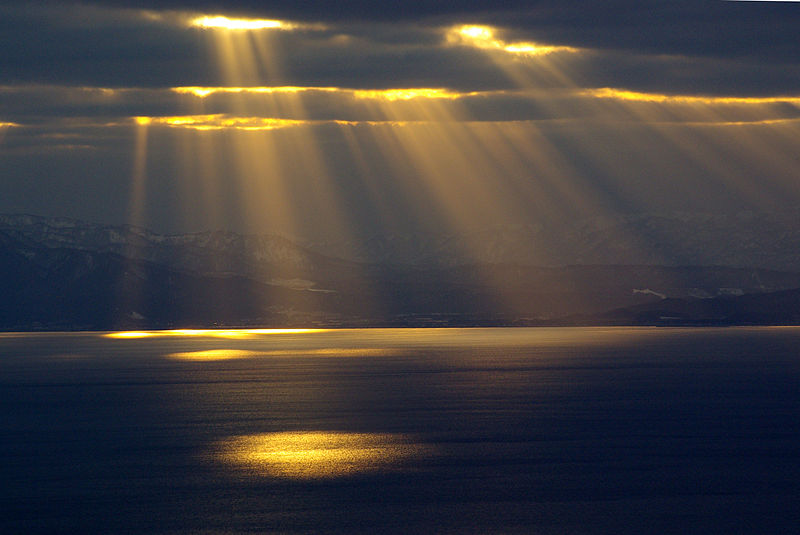
\includegraphics[scale=0.3]{CrepuscularRays.jpg}
		\end{center}
		\caption{Crepuscular rays.}
	\end{wrapfigure}
	This effect gives you astonishing and very atmospheric results while demanding little resources. As a side note, you can replace or complement the following techniques with a textured plane (\href{https://forums.unrealengine.com/showthread.php?69406-Tutorial-Godrays!}{example}) if you want an extra effect or you have a complicated lighting situation. However, to reach satisfying results with this, you need to have certain artistic skills. You can also add particle effects like steam or dust at those places, especially inside buildings.
	
	\clearpage
	
	\section*{Light Shaft Occlusion}
	The technique \textit{Light Shaft Occlusion} offers a realistic solution as the rays are created by objects blocking the path of light rays.
	\begin{wrapfigure}[5]{r}{0.5\textwidth}
		\begin{center}
			\vspace{-20px}
			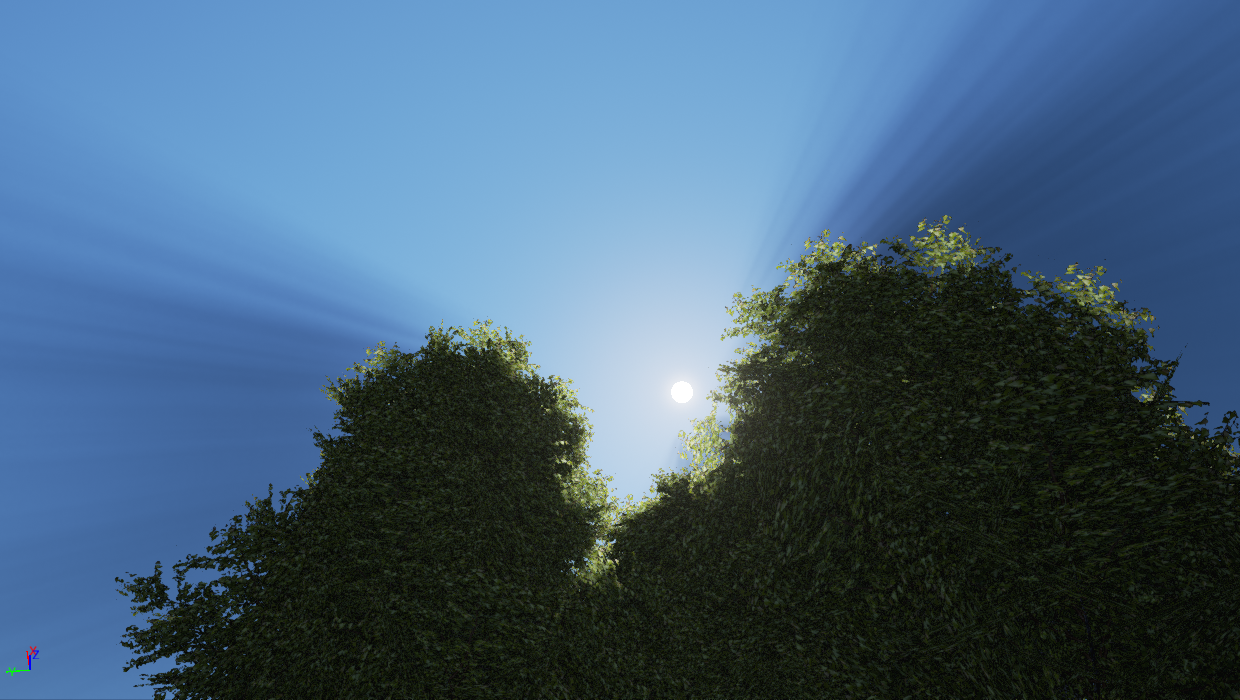
\includegraphics[scale=0.13]{Occlusion.png}
			\vspace{-20px}
		\end{center}
		\caption{Light Shaft Occlusion of a dynamic directional light with standard settings: \textit{Occlusion Mask Darkness}: \textbf{0.05}; \textit{Occlusion Depth Range}: \textbf{100,000.0}. Assets by \href{https://forums.unrealengine.com/showthread.php?59812-FREE-Foliage-Starter-Kit}{fighter5347}.}
		\begin{center}
			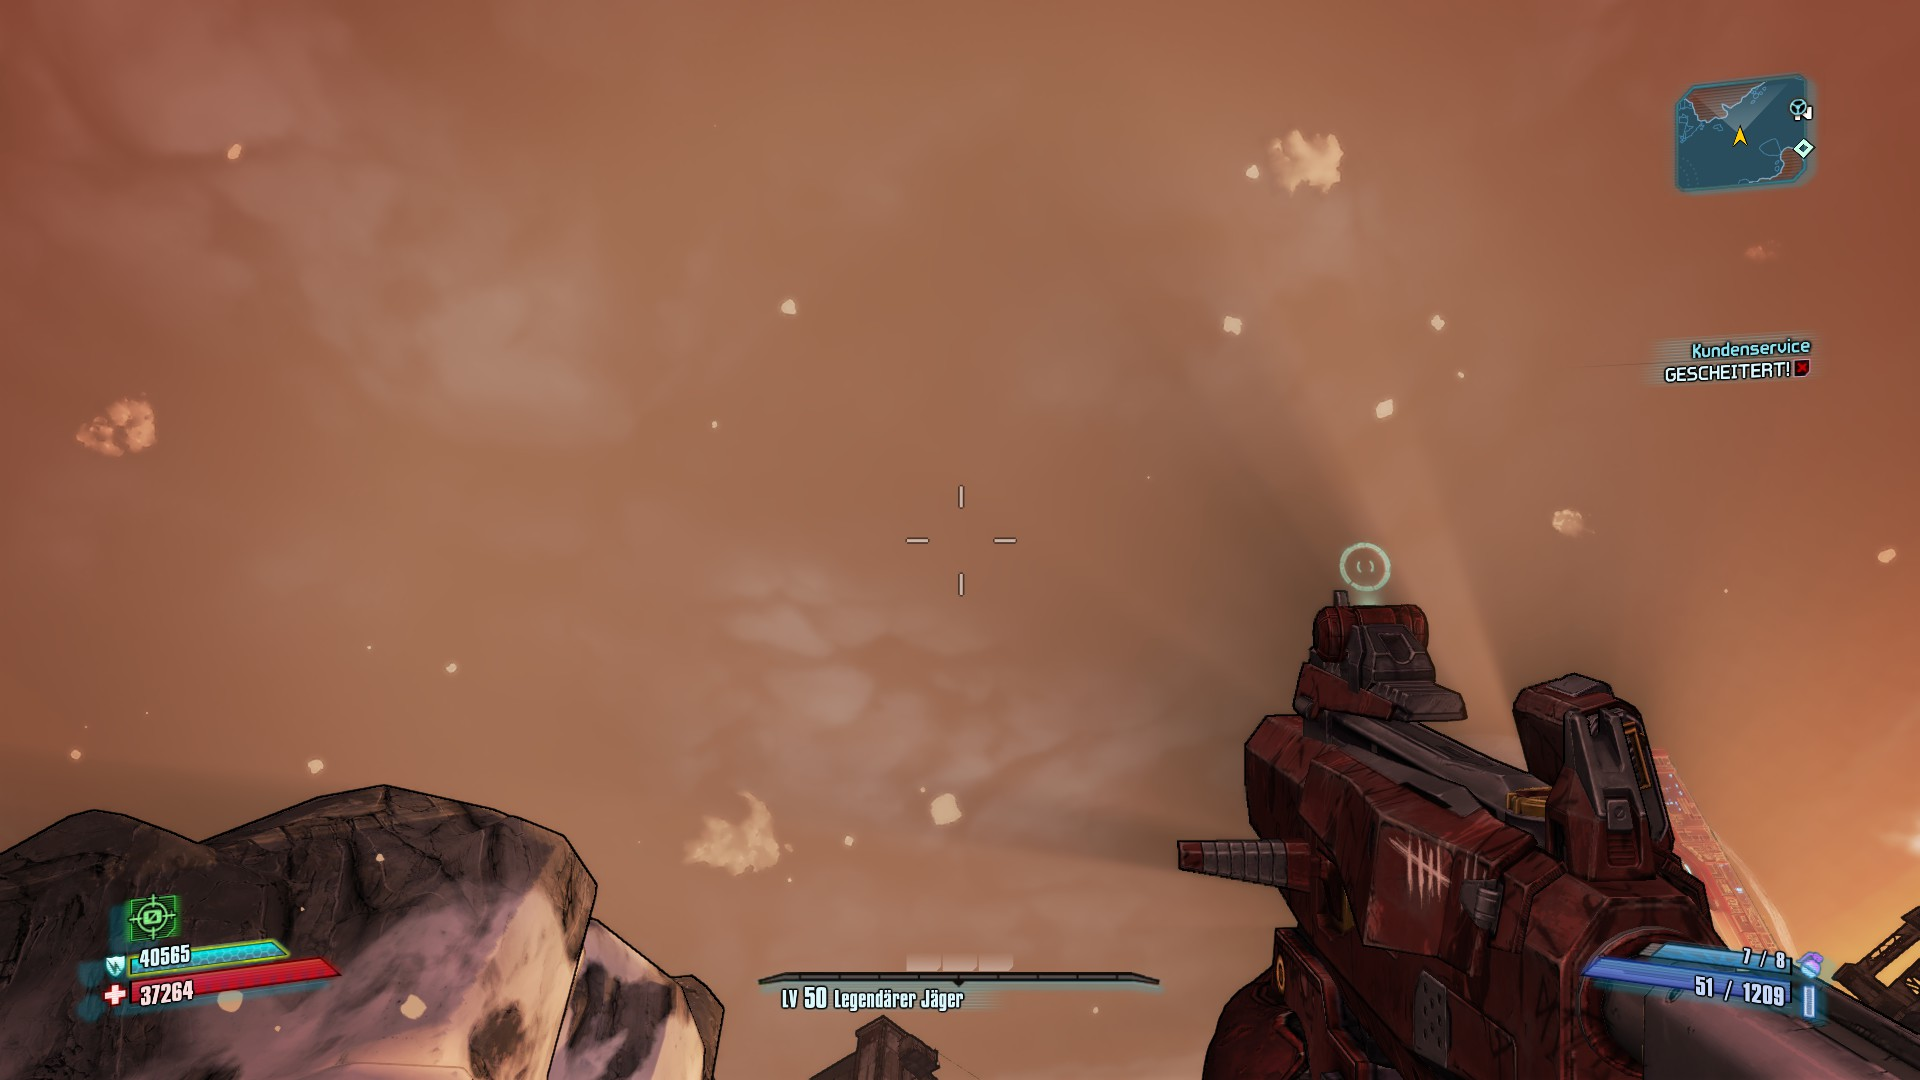
\includegraphics[scale=0.07]{Borderlands.jpg}
		\end{center}
		\vspace{-20px}
		\caption{Borderlands 2.}
		\begin{center}
			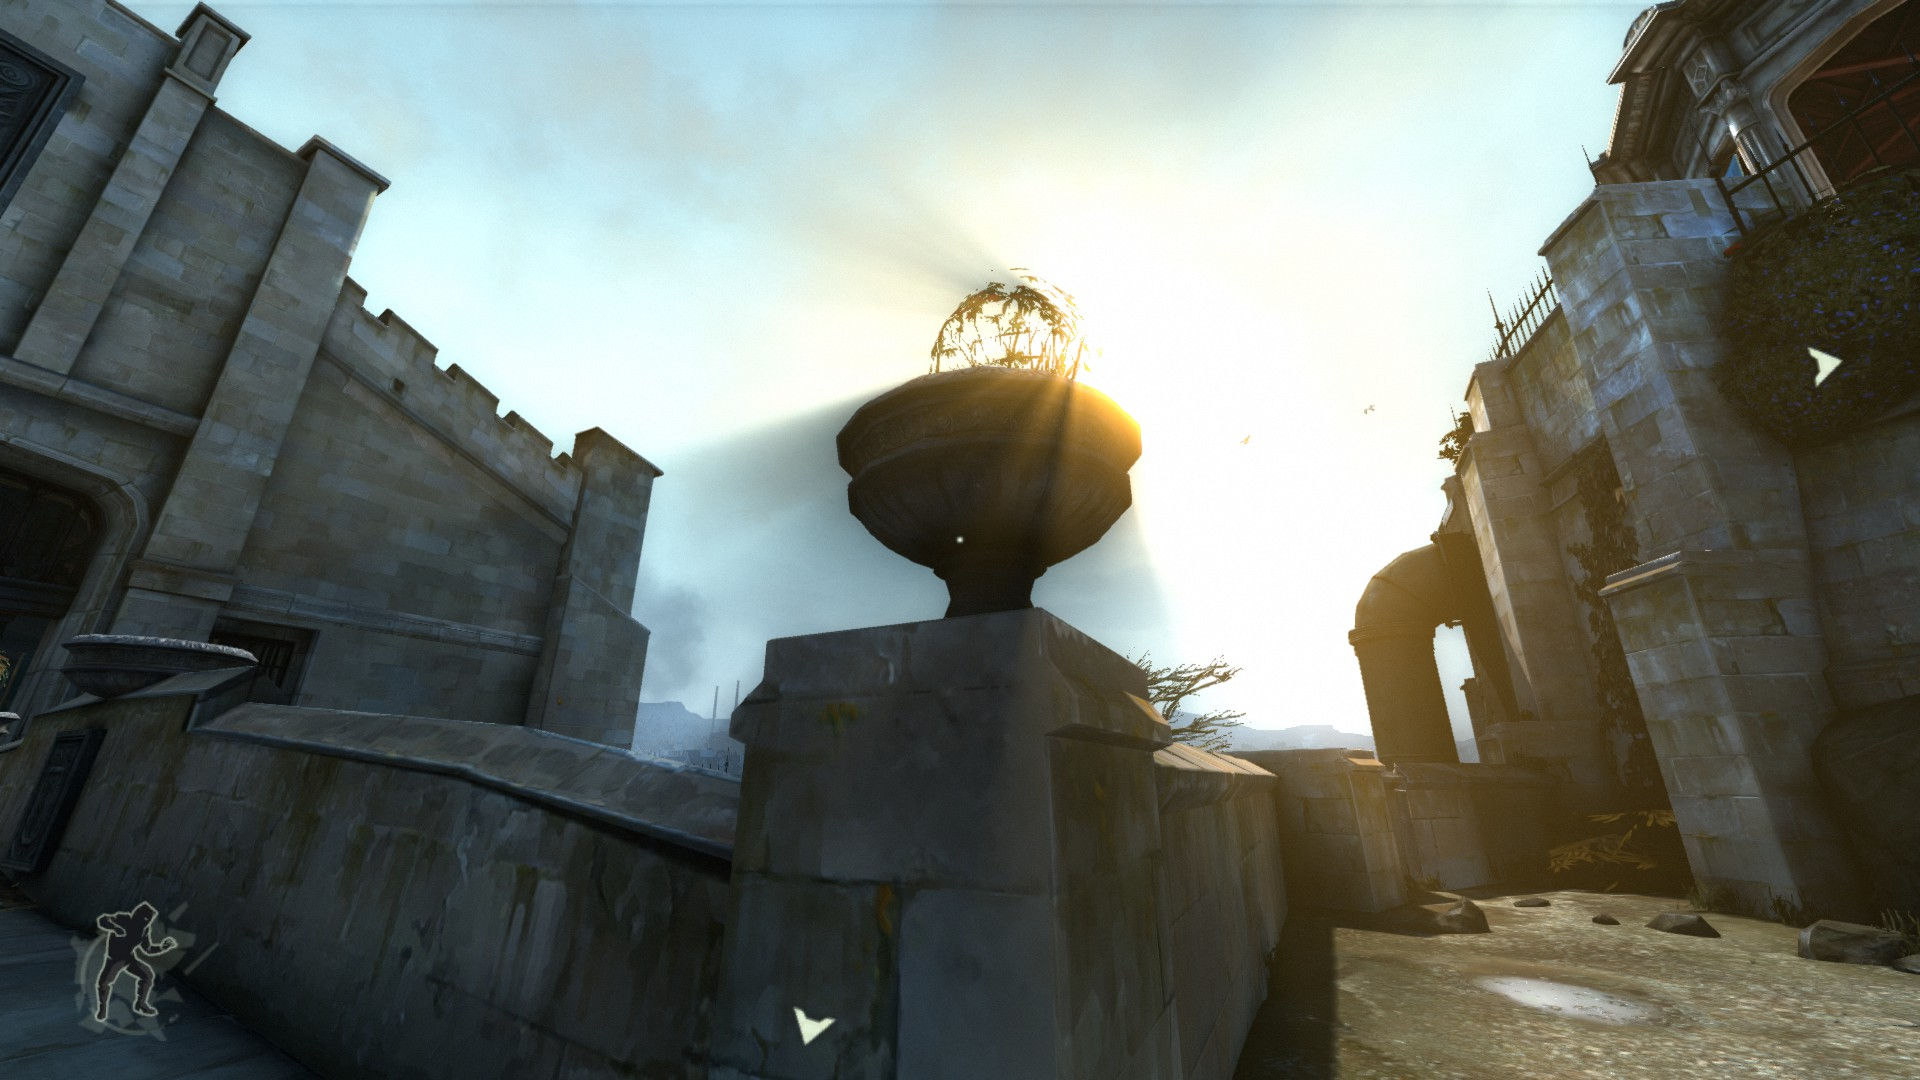
\includegraphics[scale=0.07]{Dishonored.jpg}
		\end{center}
		\vspace{-20px}
		\caption{Dishonored.}
		\begin{center}
			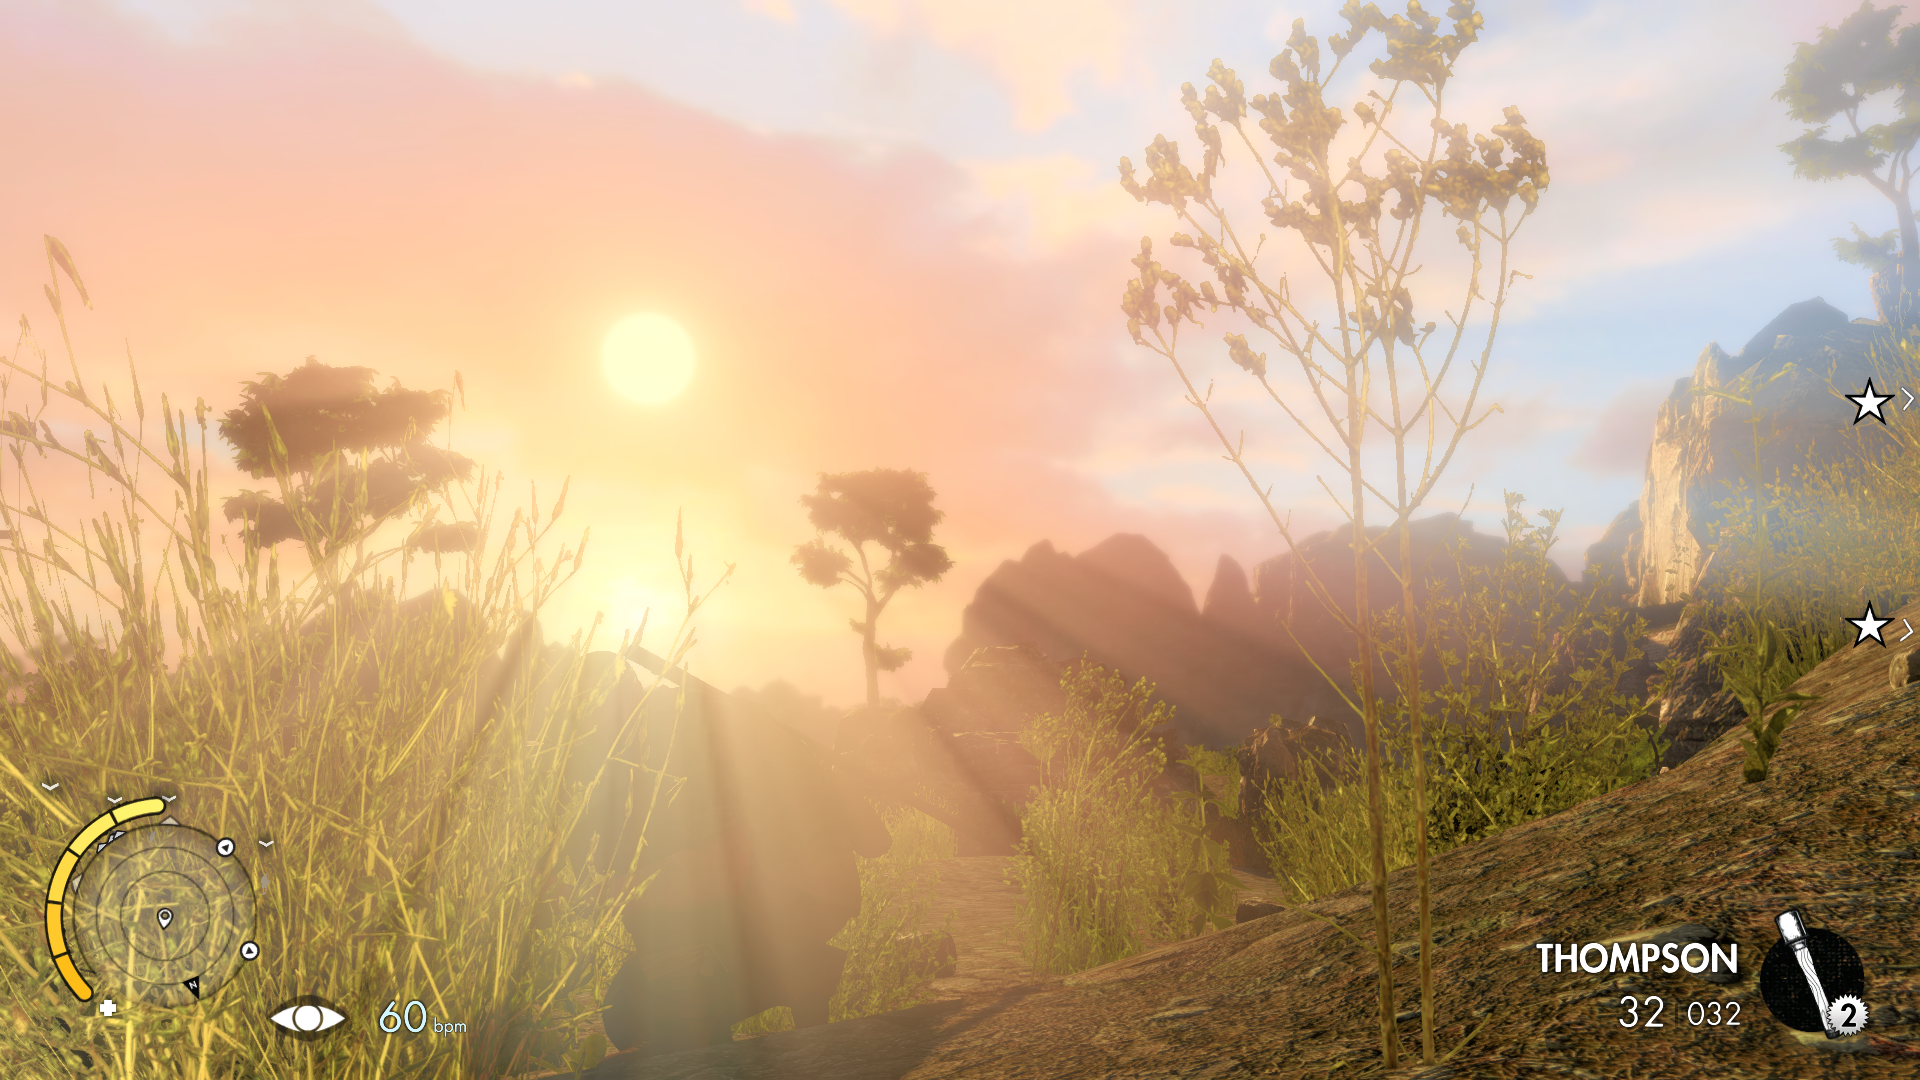
\includegraphics[scale=0.07]{SniperElite.png}
		\end{center}
		\vspace{-20px}
		\caption{Sniper Elite 3.}	
	\end{wrapfigure}
	Note that those rays can look very unrealistic if they are too dark. Then again, its strong dramatic can be used for stylized environments.
	
	\clearpage
	
	\section*{Light Shaft Bloom}
	As \href{https://docs.unrealengine.com/latest/INT/Engine/Rendering/LightingAndShadows/LightShafts/index.html#bloommethod}{the documentation} already mentions it, this method does not emulate an existant phenomenon but creates a similar effect.
	\begin{wrapfigure}[26]{r}{0.5\textwidth}
		\vspace{-20px}
		\begin{center}
			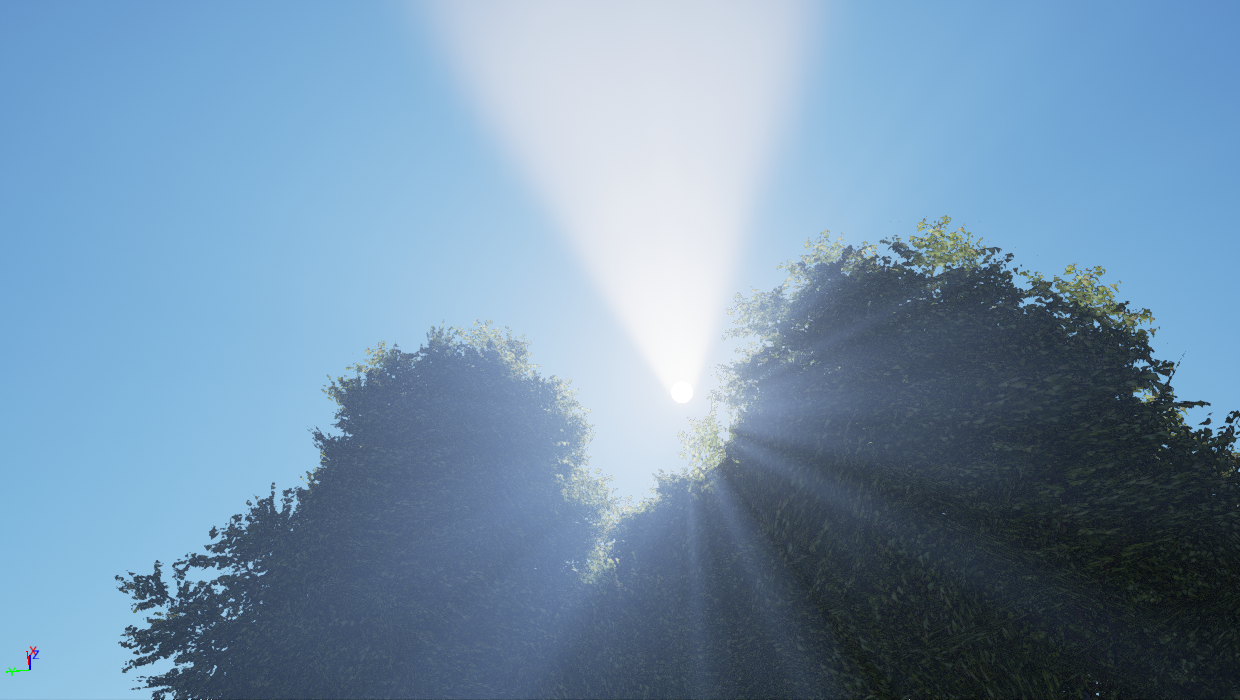
\includegraphics[scale=0.13]{Bloom.png}
		\end{center}
		\vspace{-20px}
		\caption{Light Shaft Bloom of a dynamic directional light with standard settings: \textit{Bloom Scale}: \textbf{0.2}; \textit{Bloom Treshold}: \textbf{0.0}. Assets by \href{https://forums.unrealengine.com/showthread.php?59812-FREE-Foliage-Starter-Kit}{fighter5347}.}
		\begin{center}
			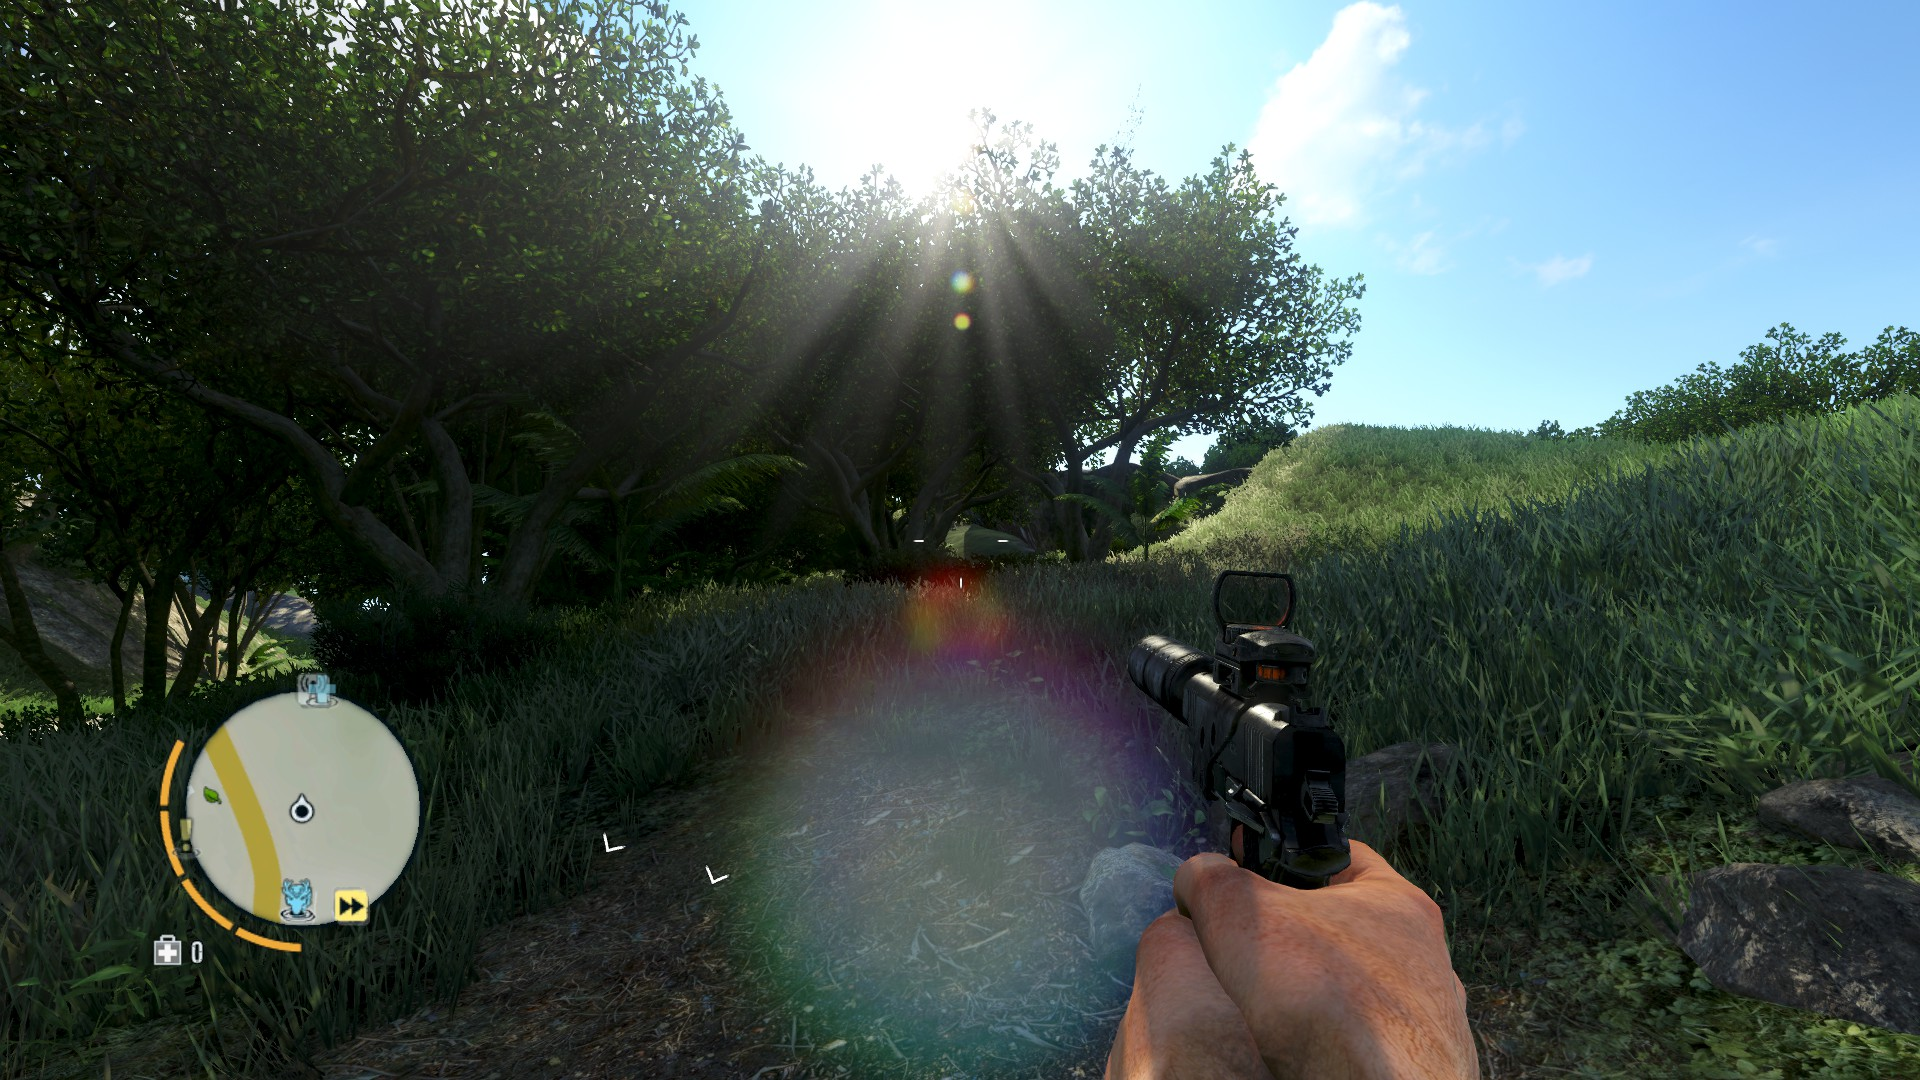
\includegraphics[scale=0.07]{FarCry.jpg}
		\end{center}
		\vspace{-20px}
		\caption{Far Cry 3.}
		\begin{center}
			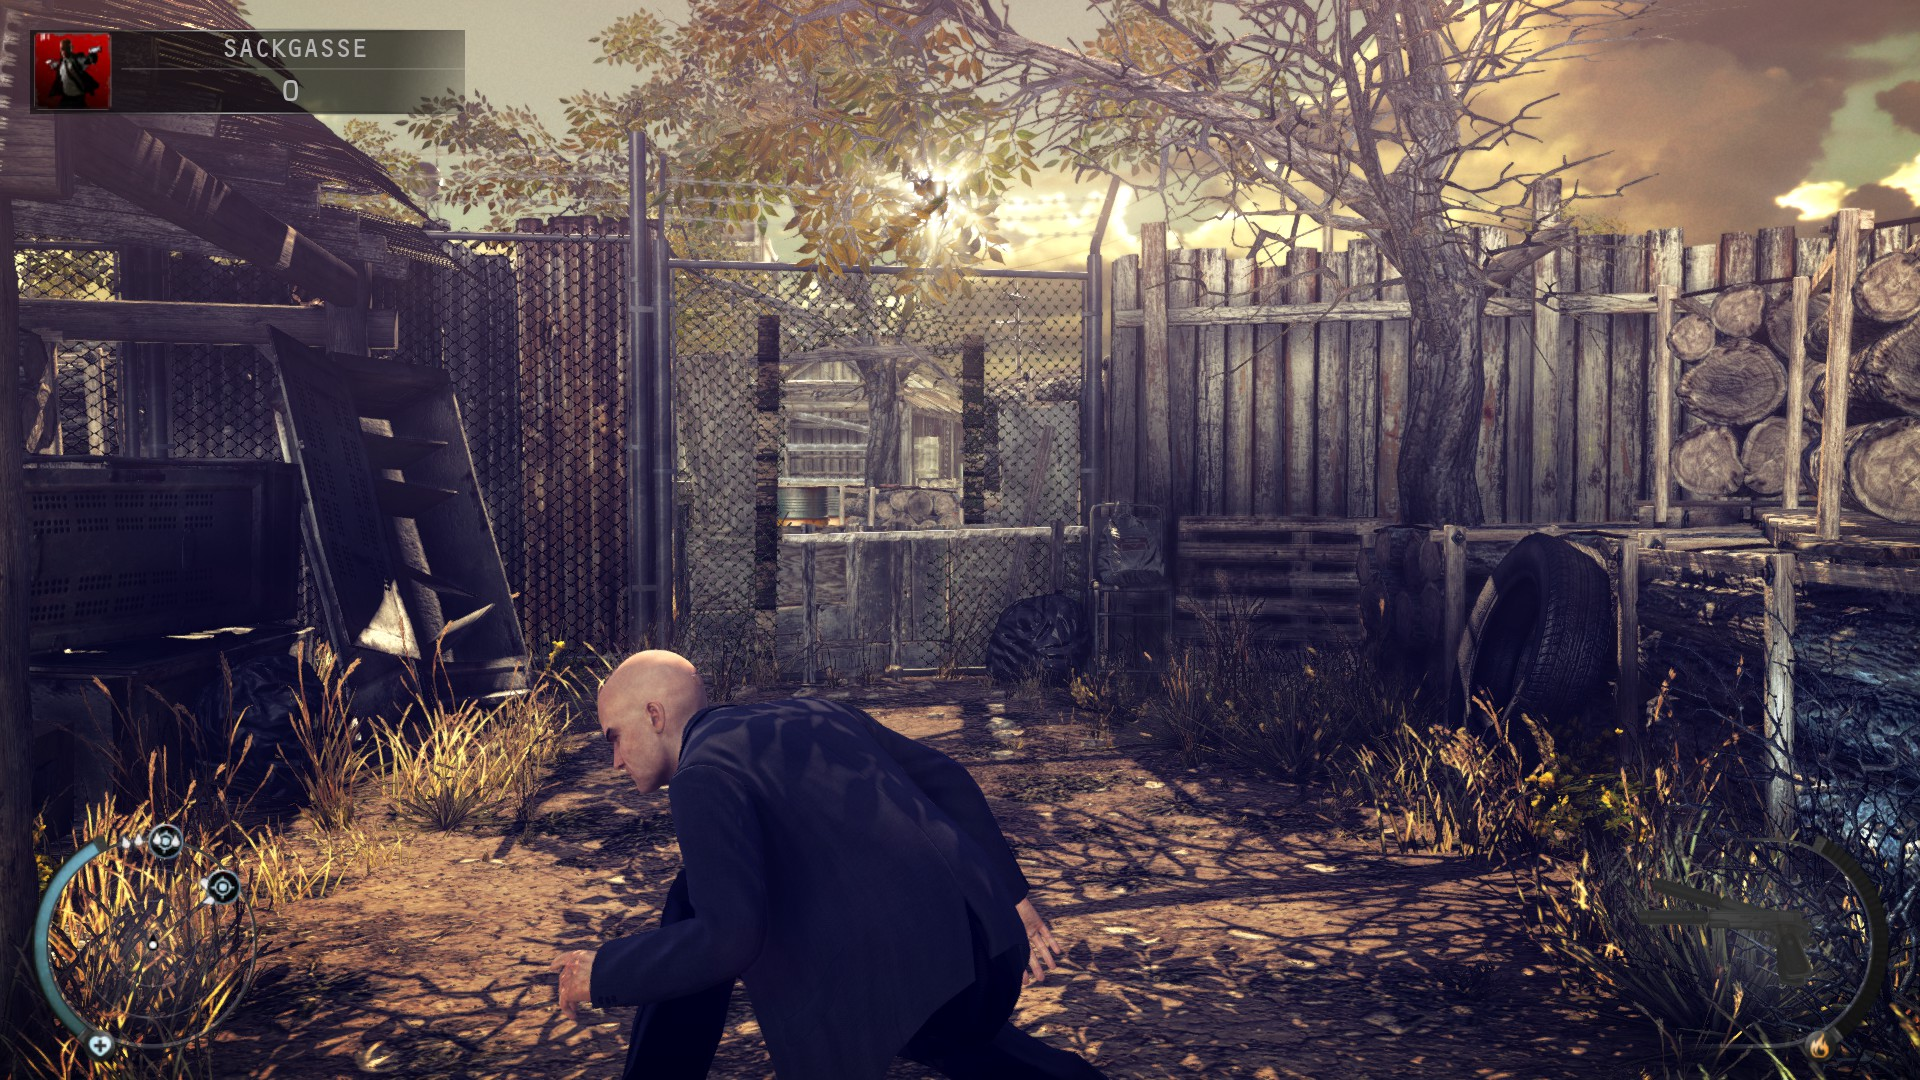
\includegraphics[scale=0.07]{Hitman.jpg}
		\end{center}
		\vspace{-20px}
		\caption{Hitman: Absolution.}
	\end{wrapfigure}
	Often enough, the light rays are using a smaller space of screen in comparison to the occlusion method, but can reach impressive results as well. The bloom methods helps in general with building a brighter and more friendly atmosphere by brightening the sky.
	
	\section*{Usage}
	\subsection*{Realistic}
	When used appropriately, Light Shafts add another layer of realism to the scene. Be aware that this realism can vanish quickly if the effect is used too often as light rays only occur at high concentrations of aerosols in the air. Realistic environments for Light Shafts include volcanic eruptions, boatages, geysers, tropical forests and foggy places in general.
	
	\subsection*{Unrealistic}
	In most games, Light Shafts are present everywhere, regardless of the environment and the given physical circumstances. That's not bad though, as light rays are a good-looking gimmick.
	
	\subsection*{Static}
	In this case, we are not talking about static lighting but the effect of light rays while the player is not moving. The Light Shafts add much more depth to the scene and make the player concentrate on the position of the directional light.
	\begin{wrapfigure}{r}{0.5\textwidth}
		\vspace{-20px}
		\begin{center}
			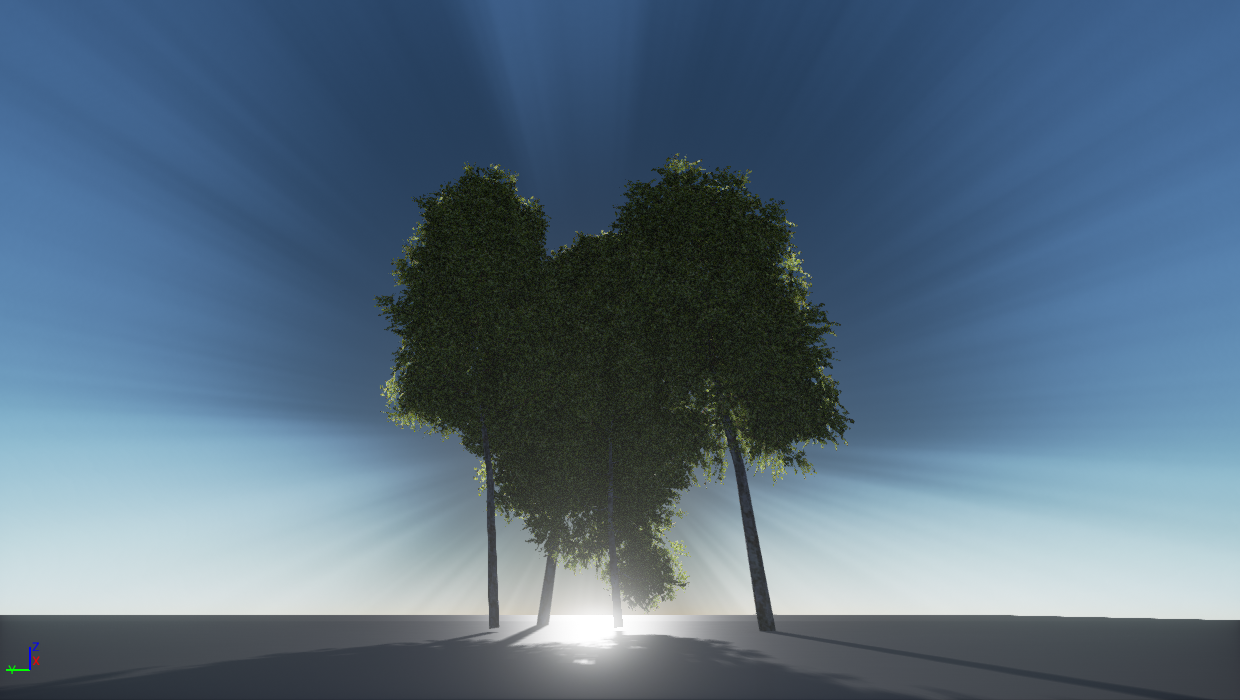
\includegraphics[scale=0.13]{OcclusionSmall.png}
		\end{center}
		\vspace{-20px}
		\caption{Standard settings with lower sun position. Assets by \href{https://forums.unrealengine.com/showthread.php?59812-FREE-Foliage-Starter-Kit}{fighter5347}.}
		\vspace{-20px}
	\end{wrapfigure}
	Additionally, light rays can stress the size of an object - it demands more space indirectly and looks much more impressive.
	
	\clearpage
	
	\subsection*{Dynamic}
	Light Shafts are especially noticeable when in motion. The first cutscene in the game \textit{Dishonored} can be used as a good example here. While in motion, the light rays move across the entire screen and make the scene look much more dynamic. This effect is also present when the player is moving independently; for example, when he is running through a thick forest and individual light rays shine through the leaf canopy.
	
	\subsection*{Combination}
	Both effects can be actived at the same time to create an interesting experience. As a result, the player just sees the shadows created by the occlusion method as long as he is standing behind a lit object, but as soon as he gets to the rim, he sees the strong light rays created by the bloom method. The mood is pretty dynamic as the contrast is amplified by the shadows and atmospheric scattering.
	
	\subsection*{Extreme Occlusion values}
	The Light Shafts look quite different if you plug in extreme values, even negative ones: Changes in perspective cause the shadows to shake around which is extremely visible as the shadows are black.
	\begin{wrapfigure}[12]{r}{0.5\textwidth}
		\vspace{-20px}
		\begin{center}
			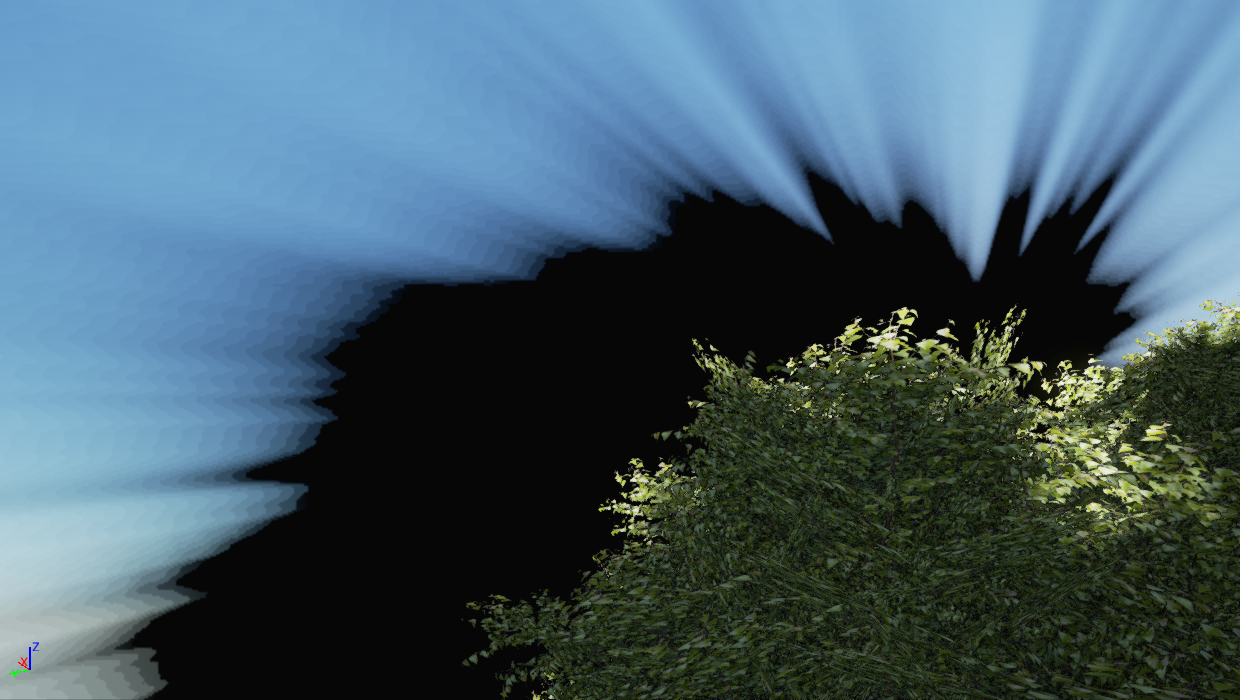
\includegraphics[scale=0.13]{OcclusionExtreme.png}
		\end{center}
		\vspace{-20px}
		\caption{Light Shaft Occlusion; \textit{Occlusion Mask Depth}: \textbf{-1.0}; \textit{Occlusion Depth Range}: \textbf{600.0}. Assets by \href{https://forums.unrealengine.com/showthread.php?59812-FREE-Foliage-Starter-Kit}{fighter5347}.}
		\vspace{-10px}
	\end{wrapfigure}
	Therefore, the scene becomes busy and unstable - an interesting effect. However, you have to note that the quality of the Light Shafts decreases: At the transistions, the colors are posterized. A further decrease of the \textit{Mask Depth} makes the black portion of the scene bigger.\\
	
	For a more subtle approach, you can soften the shadows by increasing the mask depth value.

	\clearpage

	\subsection*{Extreme Bloom values}
	High \textit{Bloom Scale} values create intense atmospheric scattering, blinding the player when he is looking in the direction of the light source.
	\begin{wrapfigure}[25]{r}{0.5\textwidth}
		\vspace{-20px}
		\begin{center}
			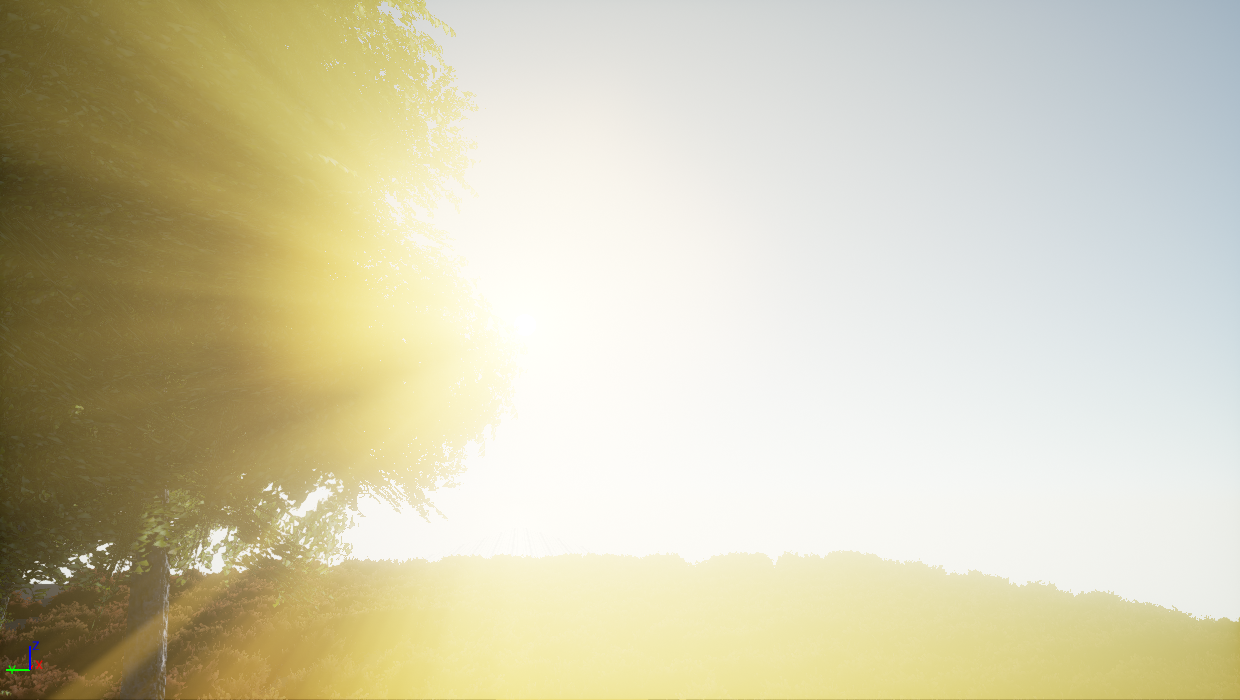
\includegraphics[scale=0.13]{BloomExtreme.png}
		\end{center}
		\vspace{-20px}
		\caption{Light Shaft Bloom; \textit{Bloom Scale}: \textbf{1.15}; \textit{Bloom Treshold}: \textbf{0.0}; \textit{Bloom Tint}: \textbf{EBB653FF}. Assets by \href{https://forums.unrealengine.com/showthread.php?59812-FREE-Foliage-Starter-Kit}{fighter5347}.}
		\begin{center}
			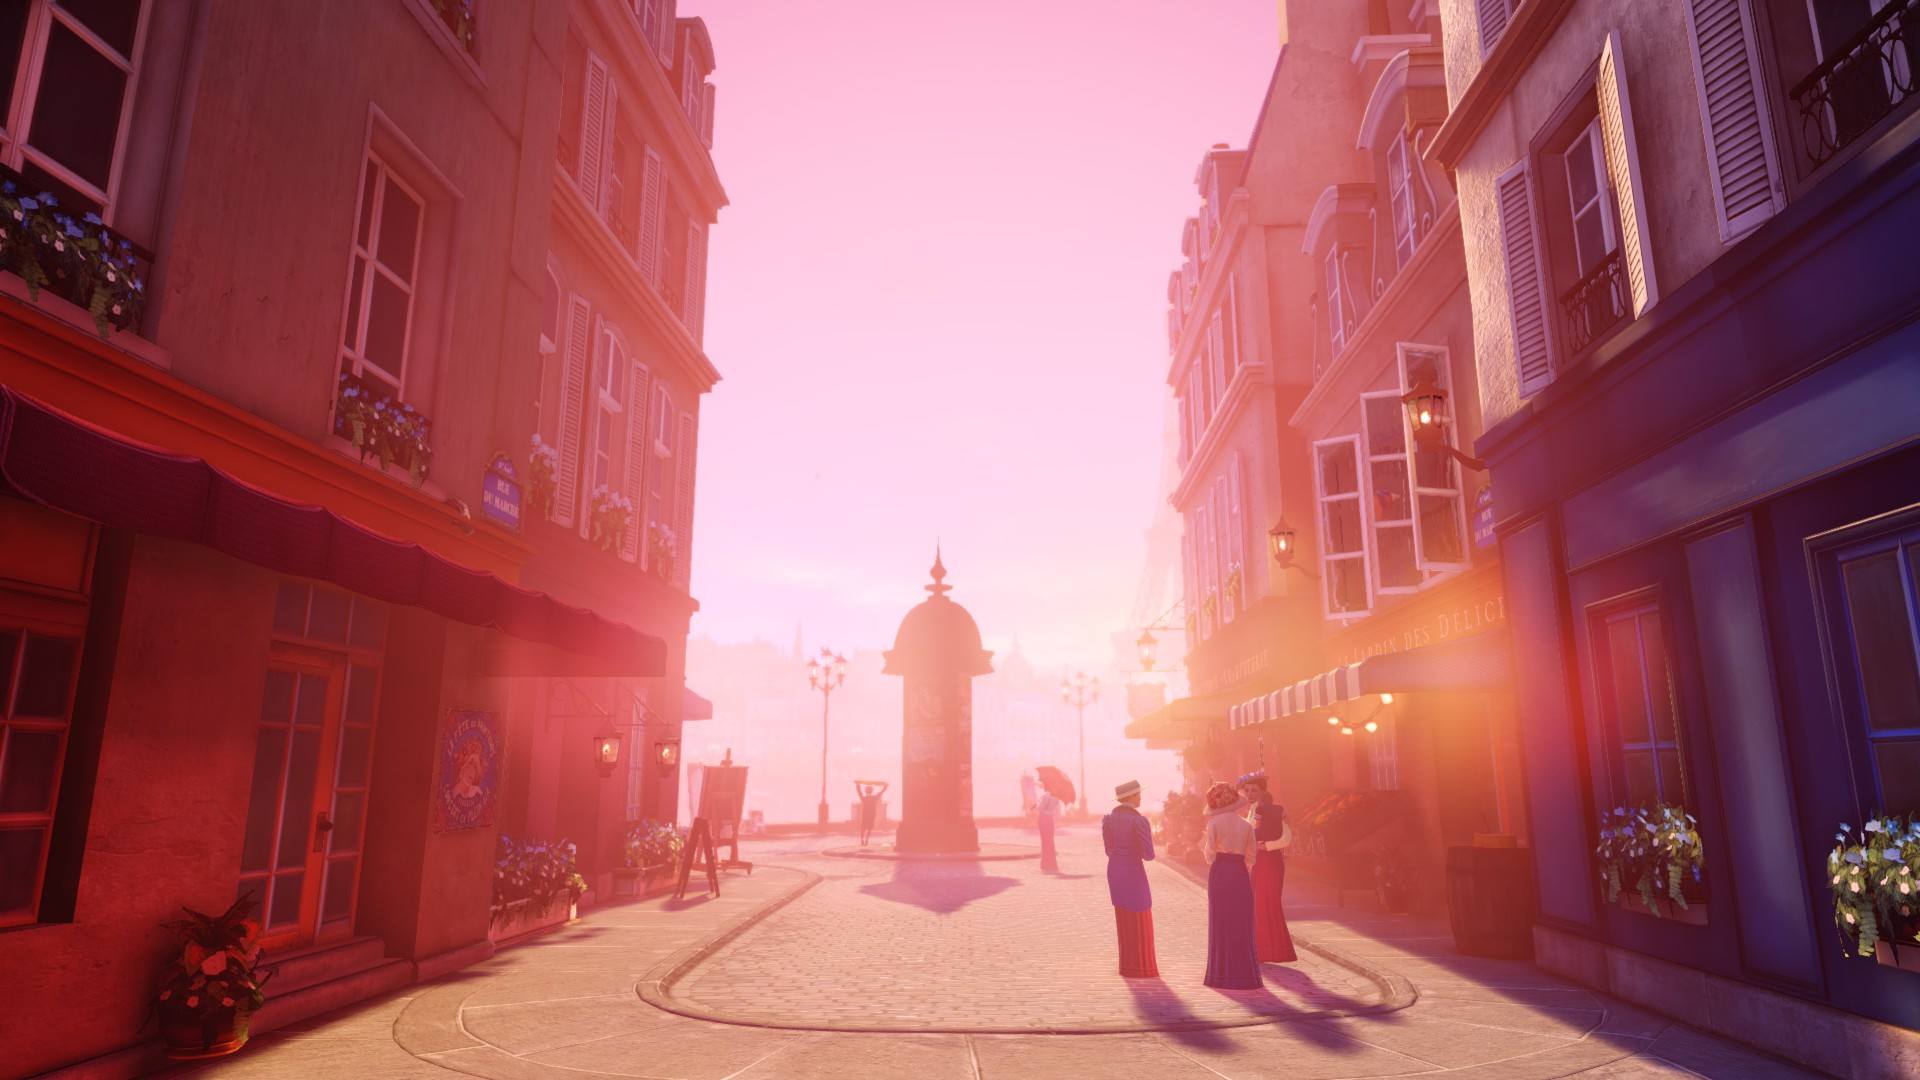
\includegraphics[scale=0.07]{Bioshock.jpg}
		\end{center}
		\vspace{-20px}
		\caption{Frontlighting creates scattering with bloom in \textit{BioShock Infinite: Burial at Sea 2}.}
	\end{wrapfigure}
	This effect can be used to create very bright and appealing landscapes. Note that if you are making the lighting very strong, the player can be disoriented quite easily - a possible use for survival-based games. Negative values in the settings do not affect anything.
	
	Furthermore, the \textit{Bloom Tint} option is worth a look as the light rays can be adapted to the overall mood - for example, you can use an orange or yellow tinge to create a good-looking dawn or dusk environment.
	
	\subsection*{Mutiple light sources}
	Even though it is often enough just the sun to create prepuscular rays in the real world, you can have much more light sources that can generate this effect.
	\begin{wrapfigure}{r}{0.5\textwidth}
		\vspace{-20px}
		\begin{center}
			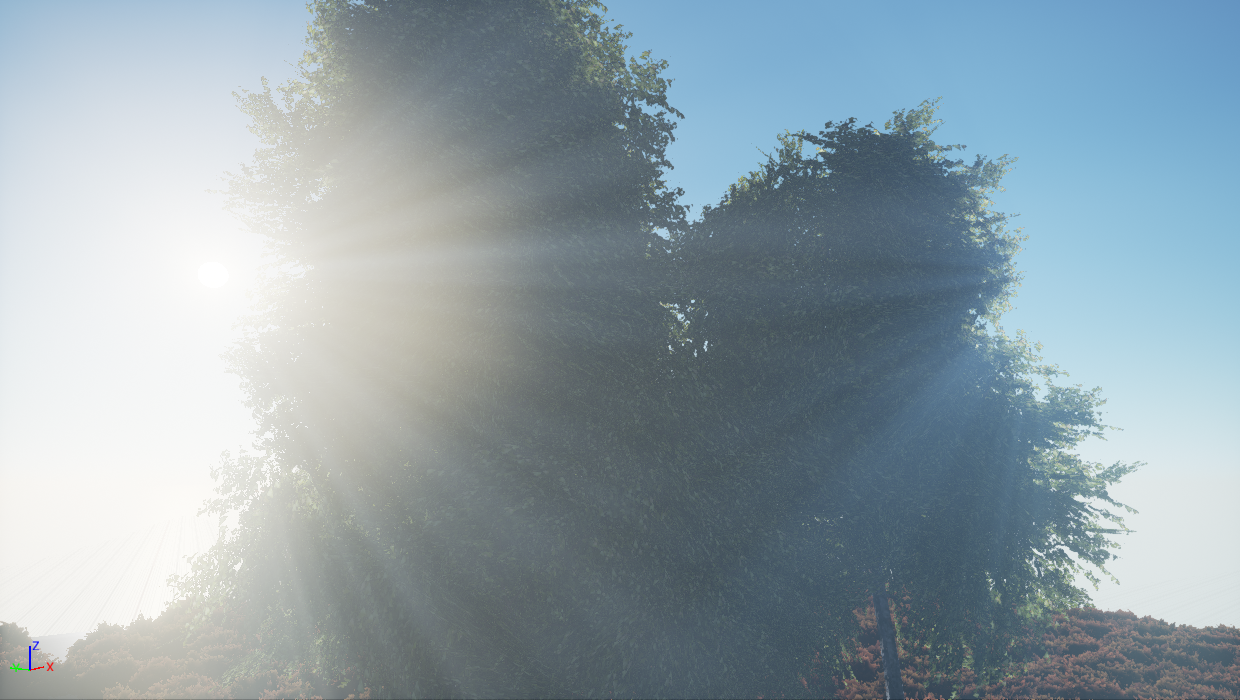
\includegraphics[scale=0.13]{MultipleLights.png}
		\end{center}
		\vspace{-20px}
		\caption{Two directional lights with actived Light Shaft Bloom and standard values. Assets by \href{https://forums.unrealengine.com/showthread.php?59812-FREE-Foliage-Starter-Kit}{fighter5347}.}
	\end{wrapfigure}
	This presentation allows an unique dynamic with a special geometry where the light rays meet. If you are considering a combination of the occlusion and bloom method, you should be aware that those effects can reverse each other partially, making them less impressive.
	
\end{document}